\section{Version control systems and Git history}

\begin{frame}
\frametitle{What are Version Control Systems?}
\begin{itemize}

    \item A way to track changes\footnote[frame]{e.g. when, what, by whom,
        and why} to groups of files
    \item Most often used in software projects
    \item Most often used to track changes to text files (but not
        exclusively)
\end{itemize}
\end{frame}

\begin{frame}[fragile]
\frametitle{What are Version Control Systems?}
\begin{itemize}
    \item Akin to a time machine: one can return to previous states of a
        project
\end{itemize}
\begin{figure}
    \centerline{%
    \includegraphics[width=0.7\textwidth]{images/The_Delorian_William_Warby_flickr.pdf}}
        \caption{\tiny \emph{The Delorian}, by William Warby, Flickr:
    \url{https://www.flickr.com/photos/wwarby/9641216546/in/photostream/}}
\end{figure}
\end{frame}

\begin{frame}[fragile]
\frametitle{What are Version Control Systems?}
    \begin{itemize}
        \item Like a safety net: accidental file deletion isn't a catastrophe
    \end{itemize}
    \begin{figure}
        \centerline{%
            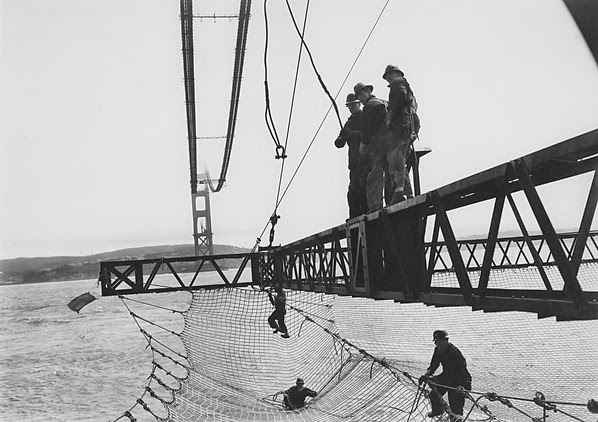
\includegraphics[height=0.65\textheight]{images/safety_net_golden_gate_bridge.jpg}}
            \caption{\tiny \url{https://todayinlaborhistory.wordpress.com/2015/01/05/january-5-1933/}}
    \end{figure}

\end{frame}

\begin{frame}[fragile]
\frametitle{What are Version Control Systems?}
    \begin{multicols}{2}
        \begin{itemize}
            \item Saved states are like anchor points in like rock climbing:
                one can fall back a small distance without losing everything
        \end{itemize}
        \begin{figure}
            \centerline{%
                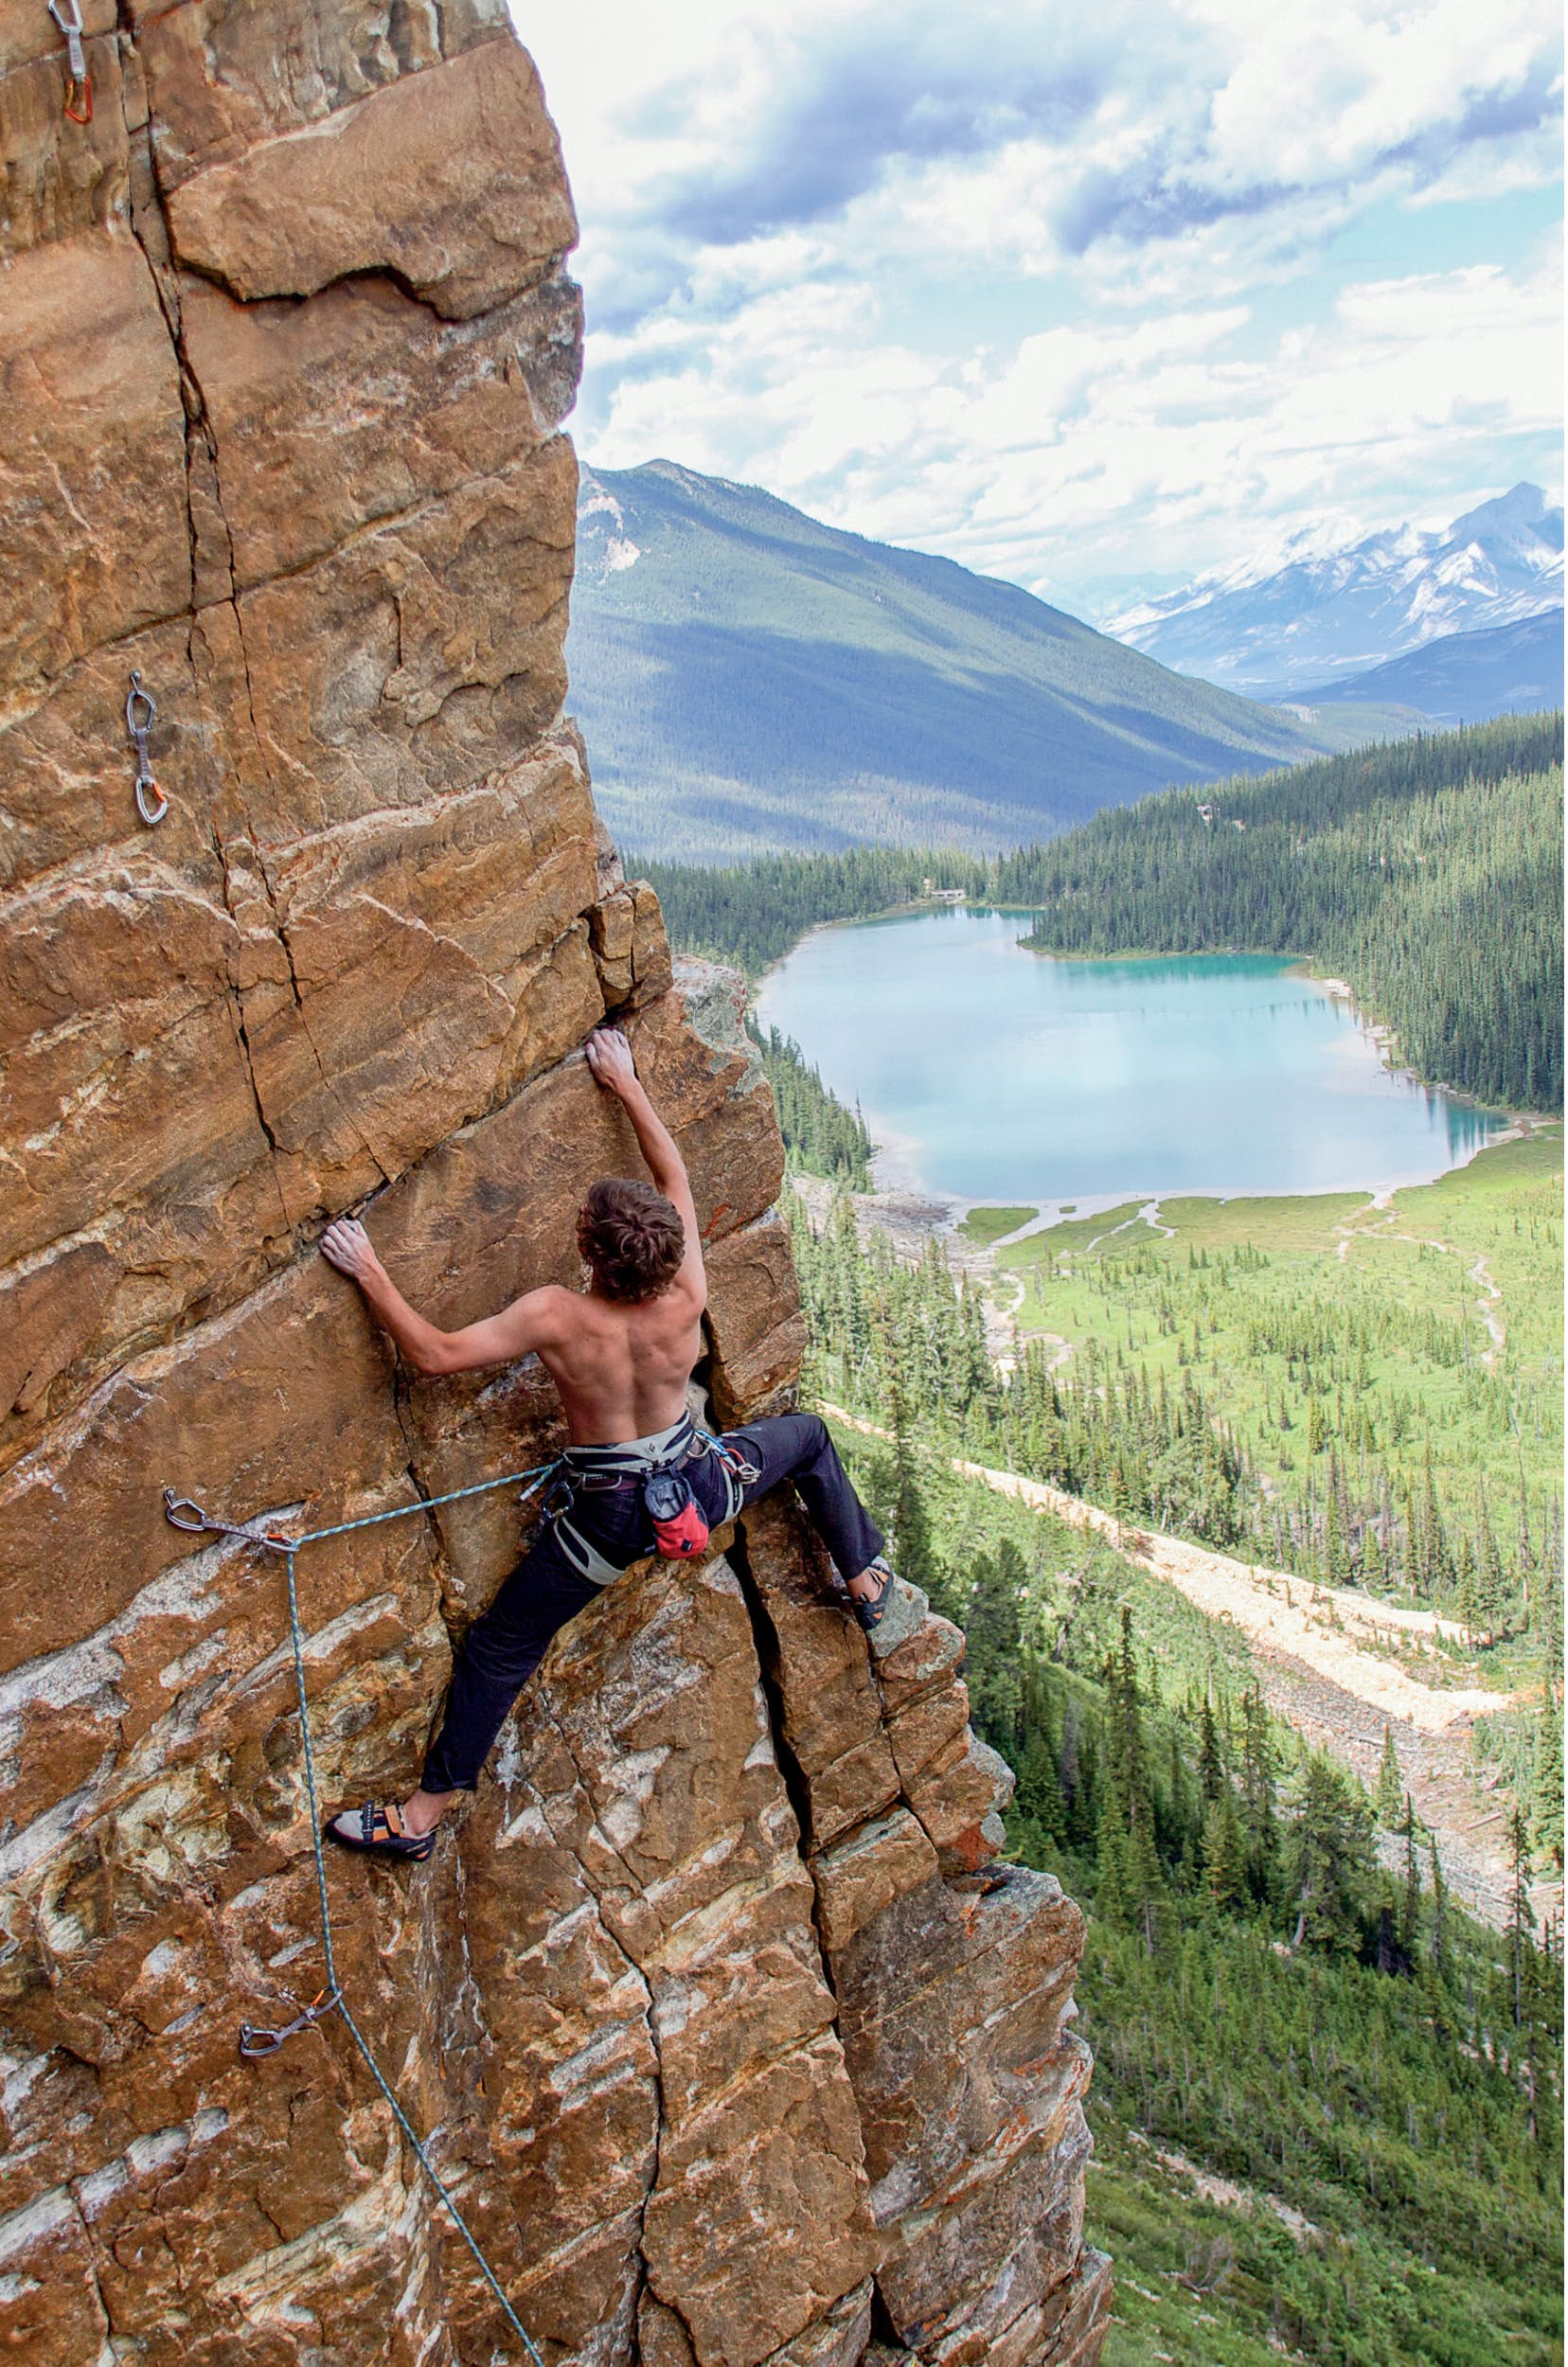
\includegraphics[height=0.8\textheight]{images/northern_exposure_jasper_rock_climbing.jpg}}
                \caption{\tiny by Fran\c{c}ois Laplante, \url{http://www.northernexposurejasper.com/}}
        \end{figure}
    \end{multicols}
\end{frame}

\begin{frame}[fragile]
\frametitle{Why use a Version Control System?}

Does this look familiar?

\begin{lstlisting}
$ ls
file.1      file.20090803  file.keep
file.2      file.alt       file.old
file.old.2  file.fixed     file.new
\end{lstlisting}
%stopzone

This is better than nothing, however \ldots
\begin{itemize}
    \item what happened between the different versions?  And just as
        important: \emph{why}?
    \item which file is actually the most current?
    \item what if \ttt{file.old} is the \emph{newest} file?
    \item can the differences between files tell us anything?
    \item why store \emph{nine} files when we really only need one?
\end{itemize}
\end{frame}

\begin{frame}
\frametitle{Why use a Version Control System?}
\begin{itemize}
    \item Version Control Systems help to tame this chaos
    \item Useful in detecting when bugs were introduced or fixed
    \item Used to save known states of a group of files and hence versions
        (releases) of a software project
    \item Can aid work on collaborative projects
\end{itemize}
\end{frame}

\begin{frame}
\frametitle{Who uses version control?}
\begin{itemize}
    \item Anyone wanting access to an old version of a document.
    \item Anyone working on a collaborative project.
    \item Anyone to whom such things have happened:
        \begin{itemize}
            \item ``It would be nice to have the version from 2 hours ago \ldots''
            \item ``I wrote that really well three days ago.  How did that
                go again?''
            \item ``Oh no!  I deleted the file!''
            \item ``Hrm, the application stopped working.  What changed in the
                last update?''
        \end{itemize}
\end{itemize}
\end{frame}

\begin{frame}
\frametitle{Where is version control used?}
    \begin{itemize}
    \item Software development
    \item Text and document processing/writing
        \begin{itemize}
            \item e.g. books, scientific articles, talks
        \end{itemize}
    \item Graphic and web design
    \item System administration
        \begin{itemize}
            \item track changes to configuration files
            \item the tool \code{etckeeper} automates this process
        \end{itemize}
    \end{itemize}
\end{frame}

        \begin{itemize}
        \end{itemize}
\end{frame}

\begin{frame}
\begin{itemize}
        \begin{itemize}
        \end{itemize}
\end{itemize}
\end{frame}

\begin{frame}
\frametitle{A short Git History}
\begin{itemize}
    \item Linux kernel development could use proprietary BitKeeper system
        free of charge
    \item The owners of BitKeeper changed the licensing conditions, which
        meant that it was no longer free for kernel developers to use
    \item Thus Linus Torvalds wrote his own system: Git
    \item Open source with a large developer community and an even larger
        user base.
\end{itemize}
\end{frame}

\begin{frame}
    \frametitle{Why use Git?}
    \begin{itemize}
        \item Supports distributed development
        \item Doesn't rely on network availability
        \item Scales to thousands of developers and millions of commits
        \item Fast!
        \item Repositories contain complete project history
        \item Lightweight branches
        \item Atomic operations
        \item Open source
        \item Free as in freedom
    \end{itemize}
\end{frame}

% vim: expandtab shiftwidth=4 softtabstop=4
